\section{Methods}\label{sec:methods}
The goal of neural network optimization is to solve an empirical risk minimization, with a loss function of the form:

\begin{equation}\label{eqn:basic_problem}
L(\theta) = \frac{1}{N} \sum_{i=1}^{N} l(x_i, \theta),
\end{equation}
where $\theta$ is the model parameters, $X$ is the training
dataset and $l(x, \theta)$ is the loss function. Here $N=|X|$ is the cardinality of the training set. In SGD, a mini-batch, $B\subset\{1,2,..., N\}$ is used to compute an (unbiased) gradient,
i.e., $g_{t} = \frac{1}{|B|} \sum_{x \in B} \nabla_\theta l(x, \theta_t)$,
and this is typically used to optimize \eqref{eqn:basic_problem} in the form:
\begin{equation}\label{eqn:sgd}
\theta_{t+1} = \theta_t - \eta_t g_t,
\end{equation}
where $\eta_t$ is the learning rate (step size) at iteration $t$, and commonly annealed during training.


By Bayes' Theorem, given the input data, $X$, a prior distribution on the model 
parameters, $P(\theta)$, and a likelihood function, $P(X|\theta)$, the posterior distribution,  $P(\theta | X)$, is:
\begin{equation}
    P(\theta | X) \propto P(\theta)P(X|\theta).
\end{equation}

From this Bayesian perspective, the goal of the neural network training is to find the Maximum-A-Posteriori (MAP) point for a given prior distribution. Note that in this context weight initialization and prior distribution are similar, that is a better prior distribution would lead to more informative posterior.
In general, it may be difficult to design a better prior given only data and a model architecture. Additionally,
the high dimensionality of the NN's parameter space renders various approaches such as adaptive priors intractable (e.g. adaptive MCMC algorithms~\cite{roberts2009examples,hu2017adaptive}).
Hence, we look into an adaptive weight ``re-initialization'' strategy. We start with an input
prior (weight initialization) and compute an approximate MAP point by annealing the noise in SGD. 
Once we compute the MAP point, we use it as a new 
initialization of the neural network weights, and restart the noise annealing 
schedule. We then iteratively repeat this process through the training process.

One approach to controlling the level of noise in SGD is via the learning rate, which is the approach used 
in~\cite{huang2017snapshot,smith2017cyclical}. However, as
discussed in~\cite{jastrzkebski2017three,smith2017don,devarakonda2017adabatch}, the batch size can also be used to control SGD noise. The motivation
for this is that larger batch sizes allow for parallel execution
which can accelerate training. 
We implement weight re-initialization through cyclical batch size schedules. 
The SGD training process is divided into one or more cycles, and in single cycle we gradually increase the batch size to decrease noise. As the noise level of SGD is annealed, $\theta$ will approaches a 
 local minima i.e., an approximate MAP point of $P(\theta| X)$.
Then at the beginning of the subsequent cycle we drop the batch size back down to the initial value, which increases the noise in SGD and "re-initializes" the neural network parameters using the previous estimate. Several CBS schedules are shown in~\fref{fig:cbs_cartoon}.

\begin{figure}[!htbp]
 \centering
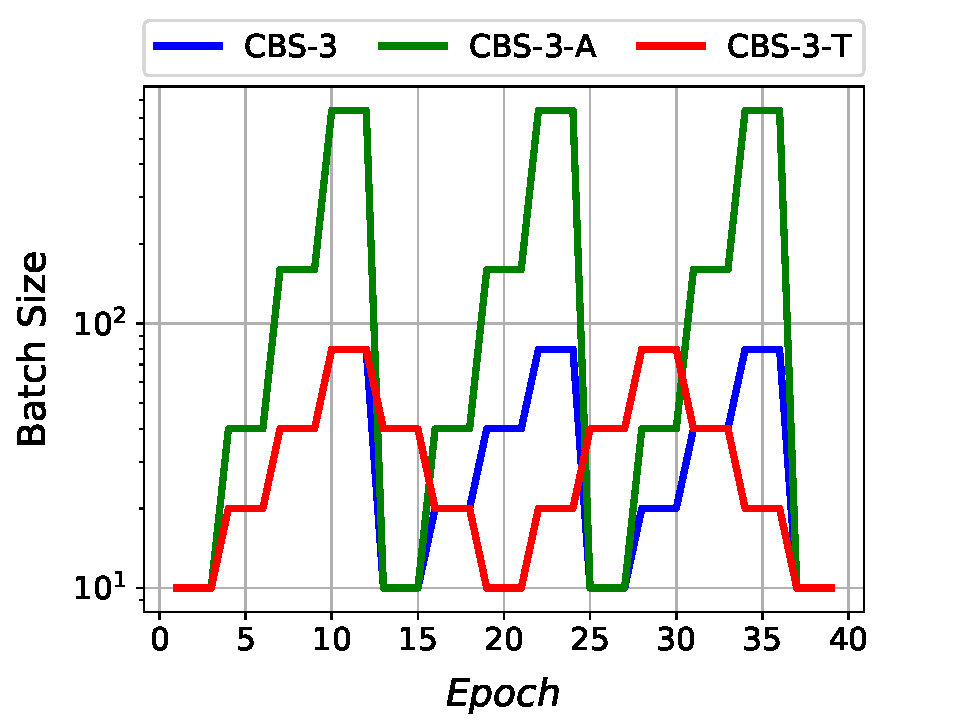
\includegraphics[width=.4\textwidth]{fig/cbs_3_cartoon.pdf}
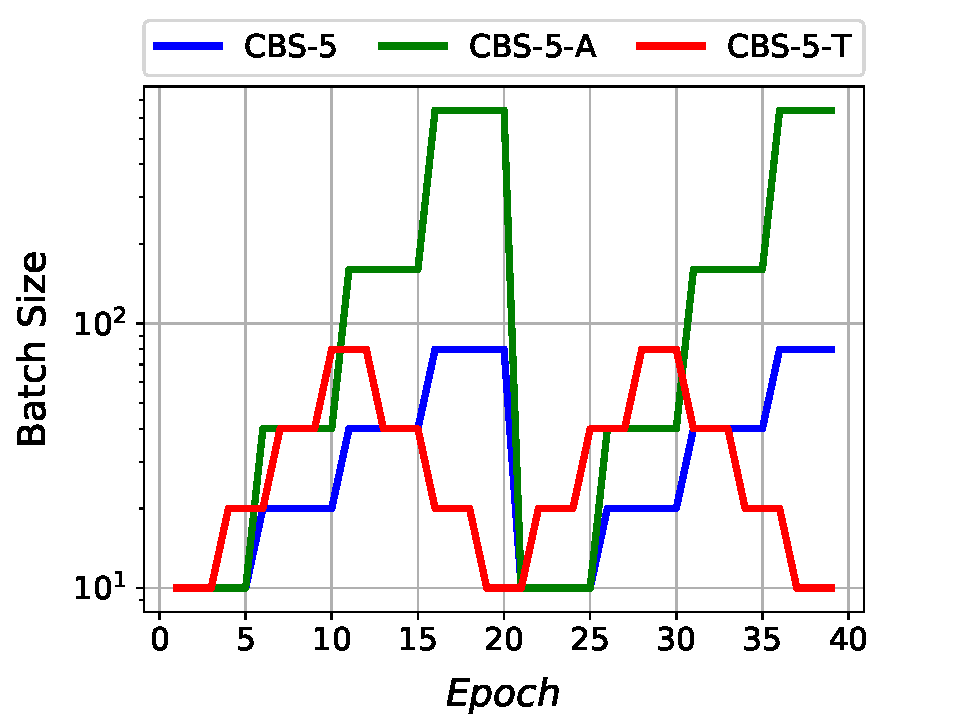
\includegraphics[width=.4\textwidth]{fig/cbs_5_cartoon.pdf}
 \caption{\footnotesize Illustration of 6 different CBS schedules, with initial batch size of 10; see Appendix~\ref{sec:training_outline} for details.} 
 \label{fig:cbs_cartoon}
\end{figure}
